\section{On the details of estimating the remote resource} \label{appendix:one-way-method}

\subsection{The importance of accounting for wave directionality}
\label{appendix:directionality}

As the National Academy review points out, estimates of $R_r$ must account for wave directionity in order to avoid double-counting. For example, when a wave with energy density of $1 \unit{kW/m}$ crosses a $1 \unit{km}$ integration contour segment with its wave crests parallel to the segment, the total power is 1MW (upper row of Figure \ref{fig:directionality}). Likewise, when that same 1-km wide wave crosses a contour-segment with its wave crests at an angle to the integration contour, the total energy contained in the wave is still only 1 MW. The directionality coefficient corrects for the fact that the length of the contour segment is longer to capture the whole 1-km wave at an angle (3 km in lower row of Figure \ref{fig:directionality}, where $\Delta\theta = \theta_n - \theta = 70.5 \unit{degrees}$). In the `unit circle' method described in the 2011 resource assessment $\delta$ is taken to be $1$ in all cases (directionality is neglected), which for the wave depicted in the lower row of Figure \ref{fig:directionality} gives an estimate of 3 MW crossing the contour. This is clearly incorrect since the 1-km wide wave only contains 1 MW of power, and demonstrates the importance of accounting for directionality.

\begin{figure}[ht]
    \centering
    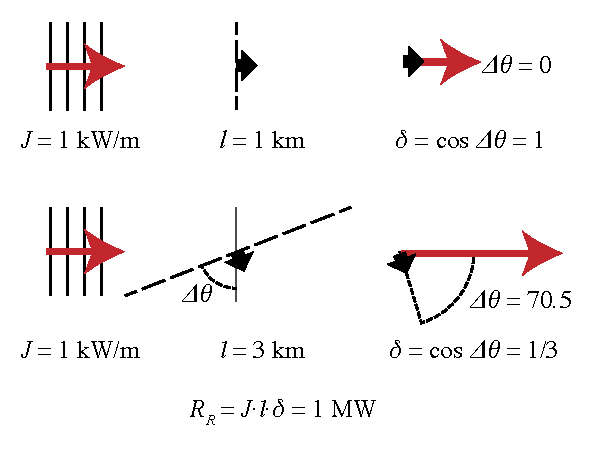
\includegraphics[width=0.6 \linewidth]{../diagram/Dot-Product_Schematic}
    \caption{A diagram depicting the importance of accounting for wave directionality. The upper sequence depicts a scenario where wave crests are parallel to the integration contour ($\delta = 1$), and the lower row is a scenario where wave crests are oblique to the contour ($\delta = 1/3$).}
    \label{fig:directionality}
\end{figure}

One of the main reasons there has been confusion about this topic is due to the fact that many types of WECs are agnostic to the direction that wave energy arrives from (Figure \ref{fig:omni-dir}A, and \cite{EPRIwaveresource2011} ). That is, all other things being equal (wave height, period, etc.), these `omnidirectional WECs' generate the same amount of power regardless of the direction that wave energy arrives from. For a single WEC of this type, it is possible to obtain an estimate of power output by simply multiplying the device's capture-width by the omnidirectional wave power. However, when many of these devices are arranged in an array where their spacing is close enough to capture all of the incident energy, then they begin to shadow one-another in a way that depends on wave direction and array-layout (i.e., in a similar manner to how wind turbine wakes reduce the performance of down-wind turbines).

Accurately modeling arrays of devices is technically challenging at regional scales, but the point here is that directionality matters for WEC arrays, and these arrays cannot generate more energy than exists in the waves. For the purposes of theoretical wave resource assessment then — instead of attempting to model arrays of devices that extract all of the energy in the wave-field — we simply draw an integration contour and assume that we can extract all of the energy that crosses it using \eqref{eqn:RR}. In other words, omnidirectional wave power is useful for quantifying the intensity of wave energy at a point and in spatial maps, but it cannot be used as a replacement for wave energy flux when performing line-integrals of the wave resource.

\begin{figure}[ht]
    \centering
    \fbox{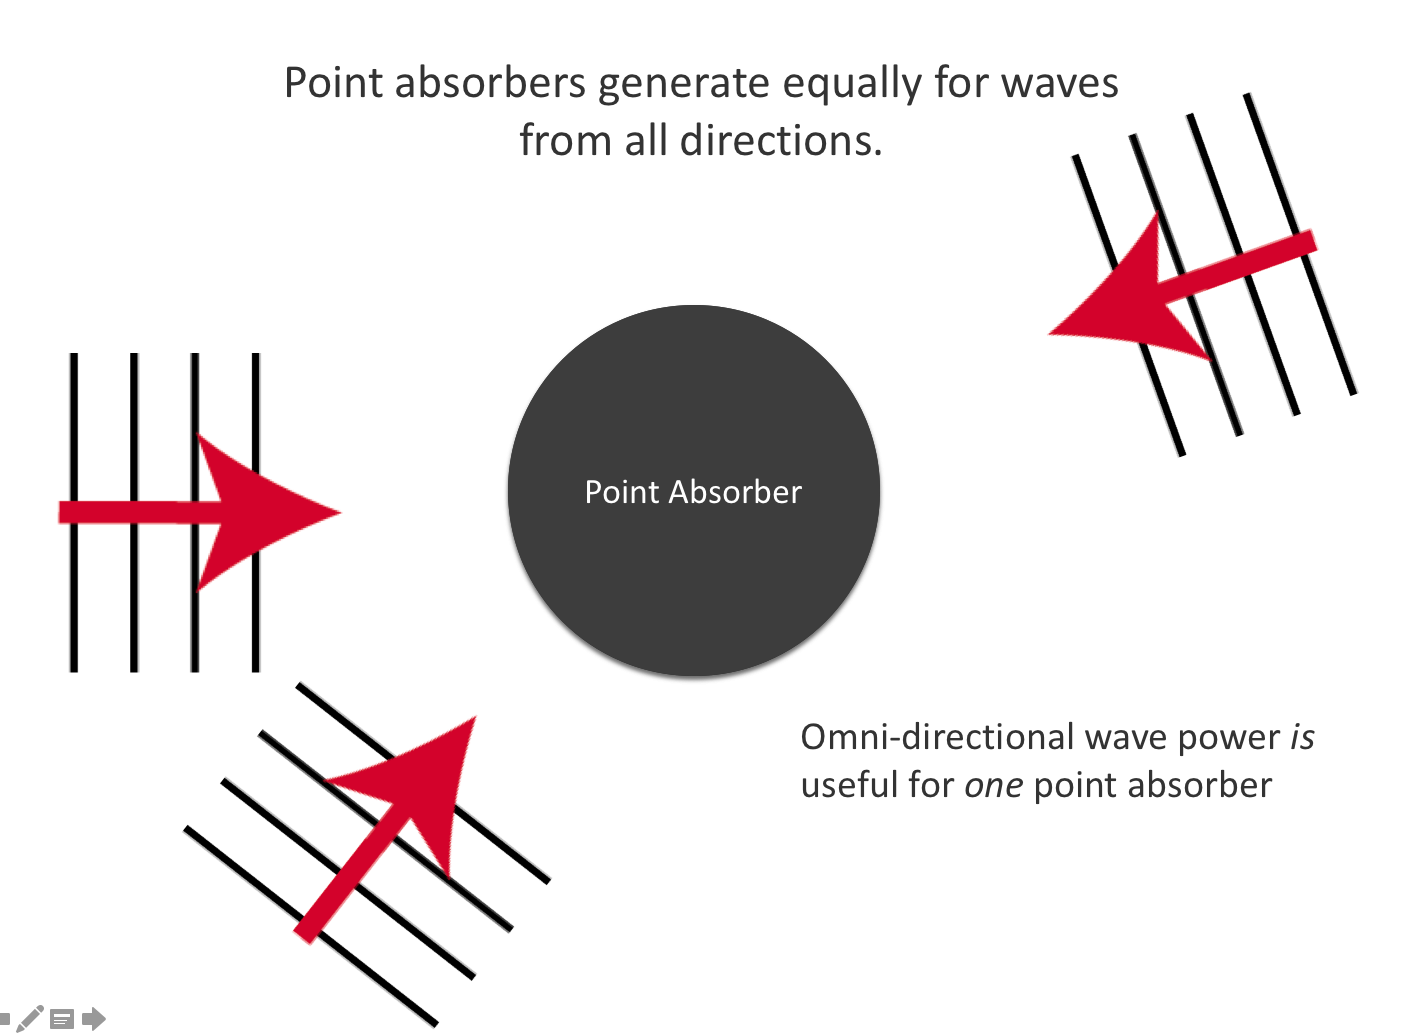
\includegraphics[width=0.3\linewidth]{../diagram/omni-dir01}}
    \fbox{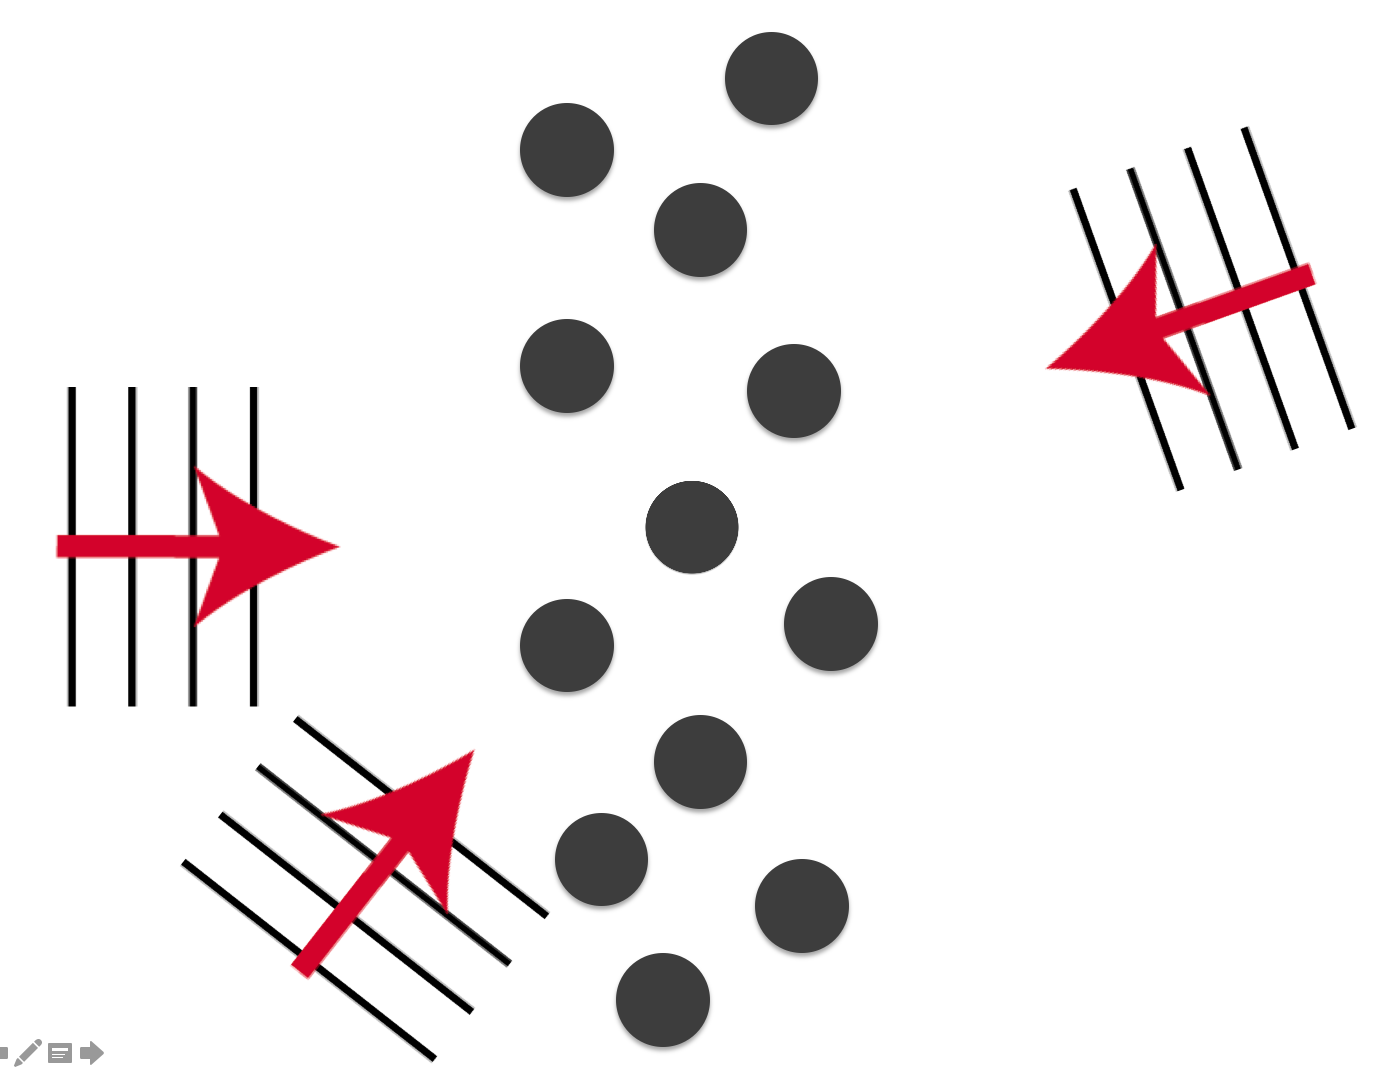
\includegraphics[width=0.3\linewidth]{../diagram/omni-dir02}}
    \fbox{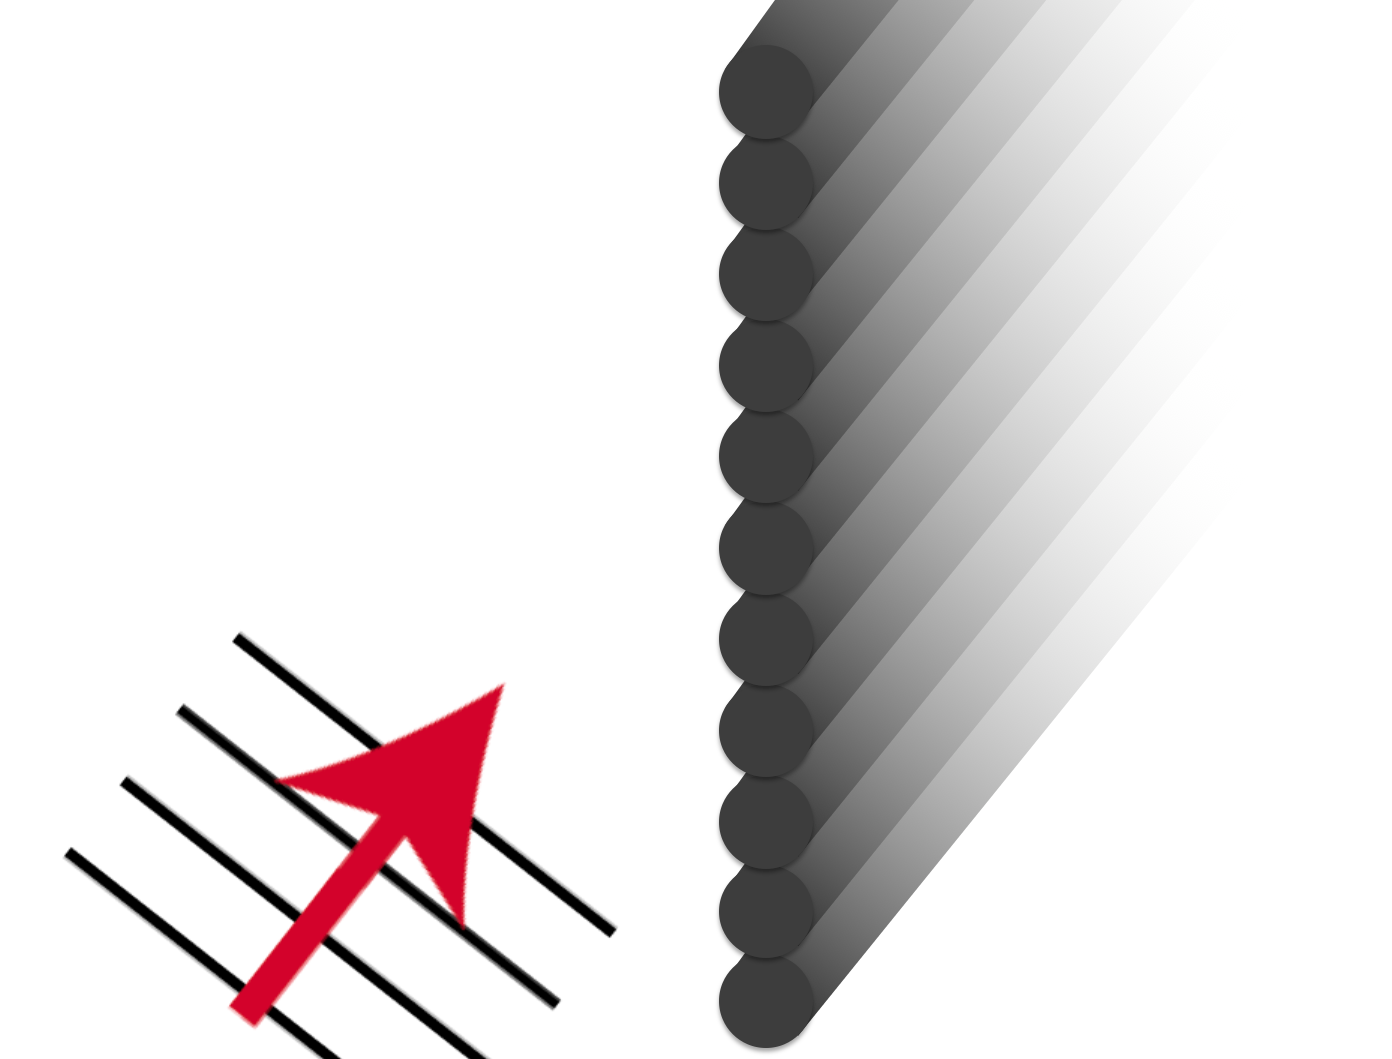
\includegraphics[width=0.3\linewidth]{../diagram/omni-dir03}}
    \caption{A) A ``point absorber'' type omni-directional WEC is denoted as a black circle. B) Though a single ``point absorber'' does not care about wave-direction, an array of such devices does because individual devices shadow one-another depending on wave direction. C) Shadowing is indicated explicitly in this case where the array is a line of ``point absorbers' spaced close enough to capture all incoming energy.\note{These figures are place-holders for now. }}
    \label{fig:omni-dir}
\end{figure}

\subsection{A detailed discussion of the `one-way' approach to estimating the remote resource}

The one-way approach to estimating $R_R$ deserves some explanation because it deviates from the traditional definition of a line-integral.

A key piece of this discussion rests on the fact that \eqref{eqn:RR} is typically computed from wave models that do not simulate the removal of the wave energy when it encounters the integration contour of interest (e.g., $\leez$). This means that, in the long time-average used in \eqref{eqn:RR}, wave energy that crosses a contour at one location may also be crossing the contour at another location at another time in the average, which can lead to over- or under-counting that wave. Without revising the model to extract the energy at the contour there is no way to know for sure whether there are waves that are being under- or over-counted in the estimate of $R_R$. Revising the model to extract wave energy that encounters the boundary, and account for it according to \eqref{eqn:RR}, is no simple task.

In a traditional line-integral the directionality coefficient is simply:
\begin{align}
    \delta_{*} = \cos(\Delta \theta)
    \label{eqn:trad-def}
\end{align}
The primary problem with this definition for the purposes of wave resource assessment is that waves that propagate away from the shoreline of interest ($|\Delta \theta | > 90$) are subtracted from the resource total. To avoid this we utilize the `one-way' condition for summing wave energy:
\begin{align}
    \delta = 
    \begin{cases}
     \delta_* & \mathrm{for\ }|\Delta \theta|<90^\circ \\
    0 & \mathrm{otherwise}.
    \end{cases}
    \label{eqn:1way-def}
\end{align}

The primary draw-back to the one-way condition is that if wave energy criss-crosses back-and-forth across the integration contour, then it is added to the total each time it crosses the contour (rather than being counted, correctly, exactly once). However, since waves do not typically swerve back and forth (i.e., across a straight line), this should only be an issue when the integration contour zig-zags or otherwise has segments that a straight-travelling wave would cross multiple times (e.g., where the contour folds, or when islands are spaced such that there are several independent contours nearby one another).

\begin{figure}[ht]
    \centering
    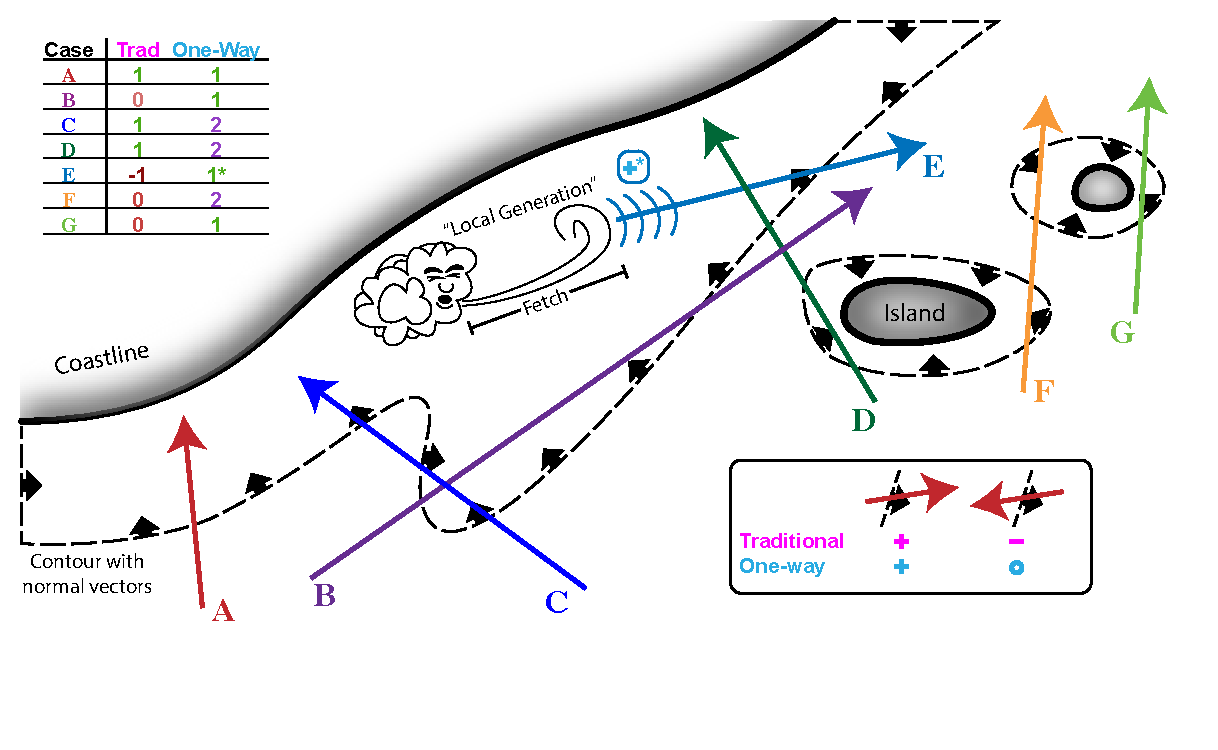
\includegraphics[width=\linewidth]{../diagram/Schematic03.pdf}
    \caption{A diagram depicting different cases of waves (color arrows) crossing an arbitrary integration contour (black dashed line). Black arrows along the contour indicate the contour-normal direction. The lower-right legend indicates whether energy is added to (+), subtracted from (-), or neglected ($\circ$) in the total where waves cross the contour. The upper-left legend indicates the `count' for each wave for the two methods. The `blowing cloud' image indicates the generation of `local waves' over the region bounded by the integration contour.}
    \label{fig:one-way-diagram}
\end{figure}

Figure \ref{fig:one-way-diagram} provides a schematic of several cases of wave energy (color arrows) propagating across an arbitrary integration contour (black dashed line). A traditional dot-product adds the energy when a wave crosses into the contour, and subtracts that energy when it passes outwards across the contour (pink row in lower right legend). The `one-way dot product' adds the energy wherever it crosses into the domain, and neglects it when it crosses outward (cyan in lower-right legend).

The arrows depict several different cases of wave energy crossing the contour. Arrow `A' indicates the most-common case of a wave crossing into the contour from offshore exactly once. Arrow `B' is a case where a wave propagates into and out-of the integration boundary. Arrow `C' is the case where a wave crosses a zig-zagging countour several times. Arrow `D' is the case of a wave propagating through an island's contour before entering the mainland contour. Arrow E is the case of a wave that is generated within the domain (i.e., locally). Arrows F and G are cases involving waves passing by islands.

The upper-left legend indicates the number of times each wave is counted using the `traditional' and the `one-way' dot-product. The correct answer is that each wave should be counted exactly once for all cases. The first thing to note, then, is that neither method gets it right in all cases. The traditional method ignores several waves, while the one-way method double-counts several. Also note here that we have included the `local resource' for arrow E (marked by $\dagger$).

What is interesting is that the one-way method is correct for several cases that would seem to be relatively common such as arrows B, E, and G. While the traditional method neglects them completely. The one-way method is only incorrect when a wave crosses a zig-zagging section of the contour (C), or when it crosses adjacent distinct contours (D, G). Therefore, as long as the integration contours are relatively straight and there are not multiple contours in close proximity, the one-way method should produce reasonably accurate results. 
The relevant length scale for defining `relatively straight' and `close proximity' is the scale over which wave energy propagates, which obviously spans ocean basins. However, it seems reasonable to assume for the EEZ boundaries we explore here, that zig-zagging is minimal and the individual boundaries are sufficiently far-apart to minimize double-counting. On the other hand, the use of the traditional dot-product is likely to result in significant under-estimation of the resource because cases E and G are very likely to occur in many scenarios. Therefore, it is straightforward to conclude that the exact answer lies somewhere between the one-way and traditional method, but in most cases is probably much closer to the latter.

We did calculate the remote resource ($R_{R*}$) using the traditional dot-product by replacing $\delta$ with $\delta_*$ in \eqref{eqn:RR}. These results show that $R_{R*}$ is smaller than $R_R$ by 20 to 100\% (Table \ref{tab:RR*}). This can be explained for most regions by assuming that 40-60\% of the locally generated waves propagate offshore. In Hawaii, where that approach does not work, the answer is clearly that a large fraction of the wave energy simply passes into and back-out-of the domain, and therefore erroneously ignored by the traditional dot-product.

\note{Should we use this analysis to estimate uncertainty in $R_R$?! ... maybe reduce $R_R$ by 10\% with a 10\% uncertainty? ... Or assume that 20\% of difference between $R_R$ and $R_{R*}$ is double-counting in $R_R$? There is also the possibility of computing 'duplication factors (fn of theta)' for the one-way method at every point along the contour, or for each domain?}

\begin{table}[ht]
  \centering
  \begin{tabular}{|c|c|c|c|}
  Region & $R_R$ & $R_{R*}$ & $R_{L\circ}$ \\
  \hline
  Alaska & 1040 & 430 & 990 \\
  West Coast & 420 & 360 & 90 \\
  Hawaii & 370 & 80 & 10 \\
  East Coast & 110 & 0 & 180 \\
  Gulf of Mexico & 13 & -2 & 56 \\
  P.R. \& U.S.V.I. & 6 & 4 & 11 \\
  \end{tabular}
  \label{tab:RR*}
  \caption{A comparison of remote resource computed using the one-way method ($R_R$) to a traditional dot-product ($R_{R*}$), and the local resource. All values in TWh/yr.}
\end{table}

The only way to avoid this error completely is to extract wave energy in the model simulation at the integration contour of interest -- and account for it according to \eqref{eqn:RR} -- so that it does not propagate to a different point on the contour where it could be mis-counted. This approach, however, is technically challenging and reduces the flexibility of data analysis because a new simulation must be run for each contour of interest.

\subsection{On the proximity of regional domains}

The issue of `double counting' arises again with this method, as discussed above, when two or more nation's EEZs are in close proximity to one another, but not quite touching. The gulf of Mexico provides an example of this: Mexico's EEZ pushes up against the U.S. EEZ. Clearly the majority of wave energy propogating north across the U.S.'s southern EEZ boundary originated within Mexico's EEZ, and therefore is technically Mexico's resource. In this case, the U.S.'s remote resource in the gulf is less than 20\% of its local resource, so it does not play a major role in the total there, nor does it contribute significantly to the nation's resource. In other cases, where the resource from a neighboring nation's EEZ might be significant, perhaps the simplest thing would be to enforce zero winds over their EEZ in the model simulation.

\begin{figure}
    \centering
    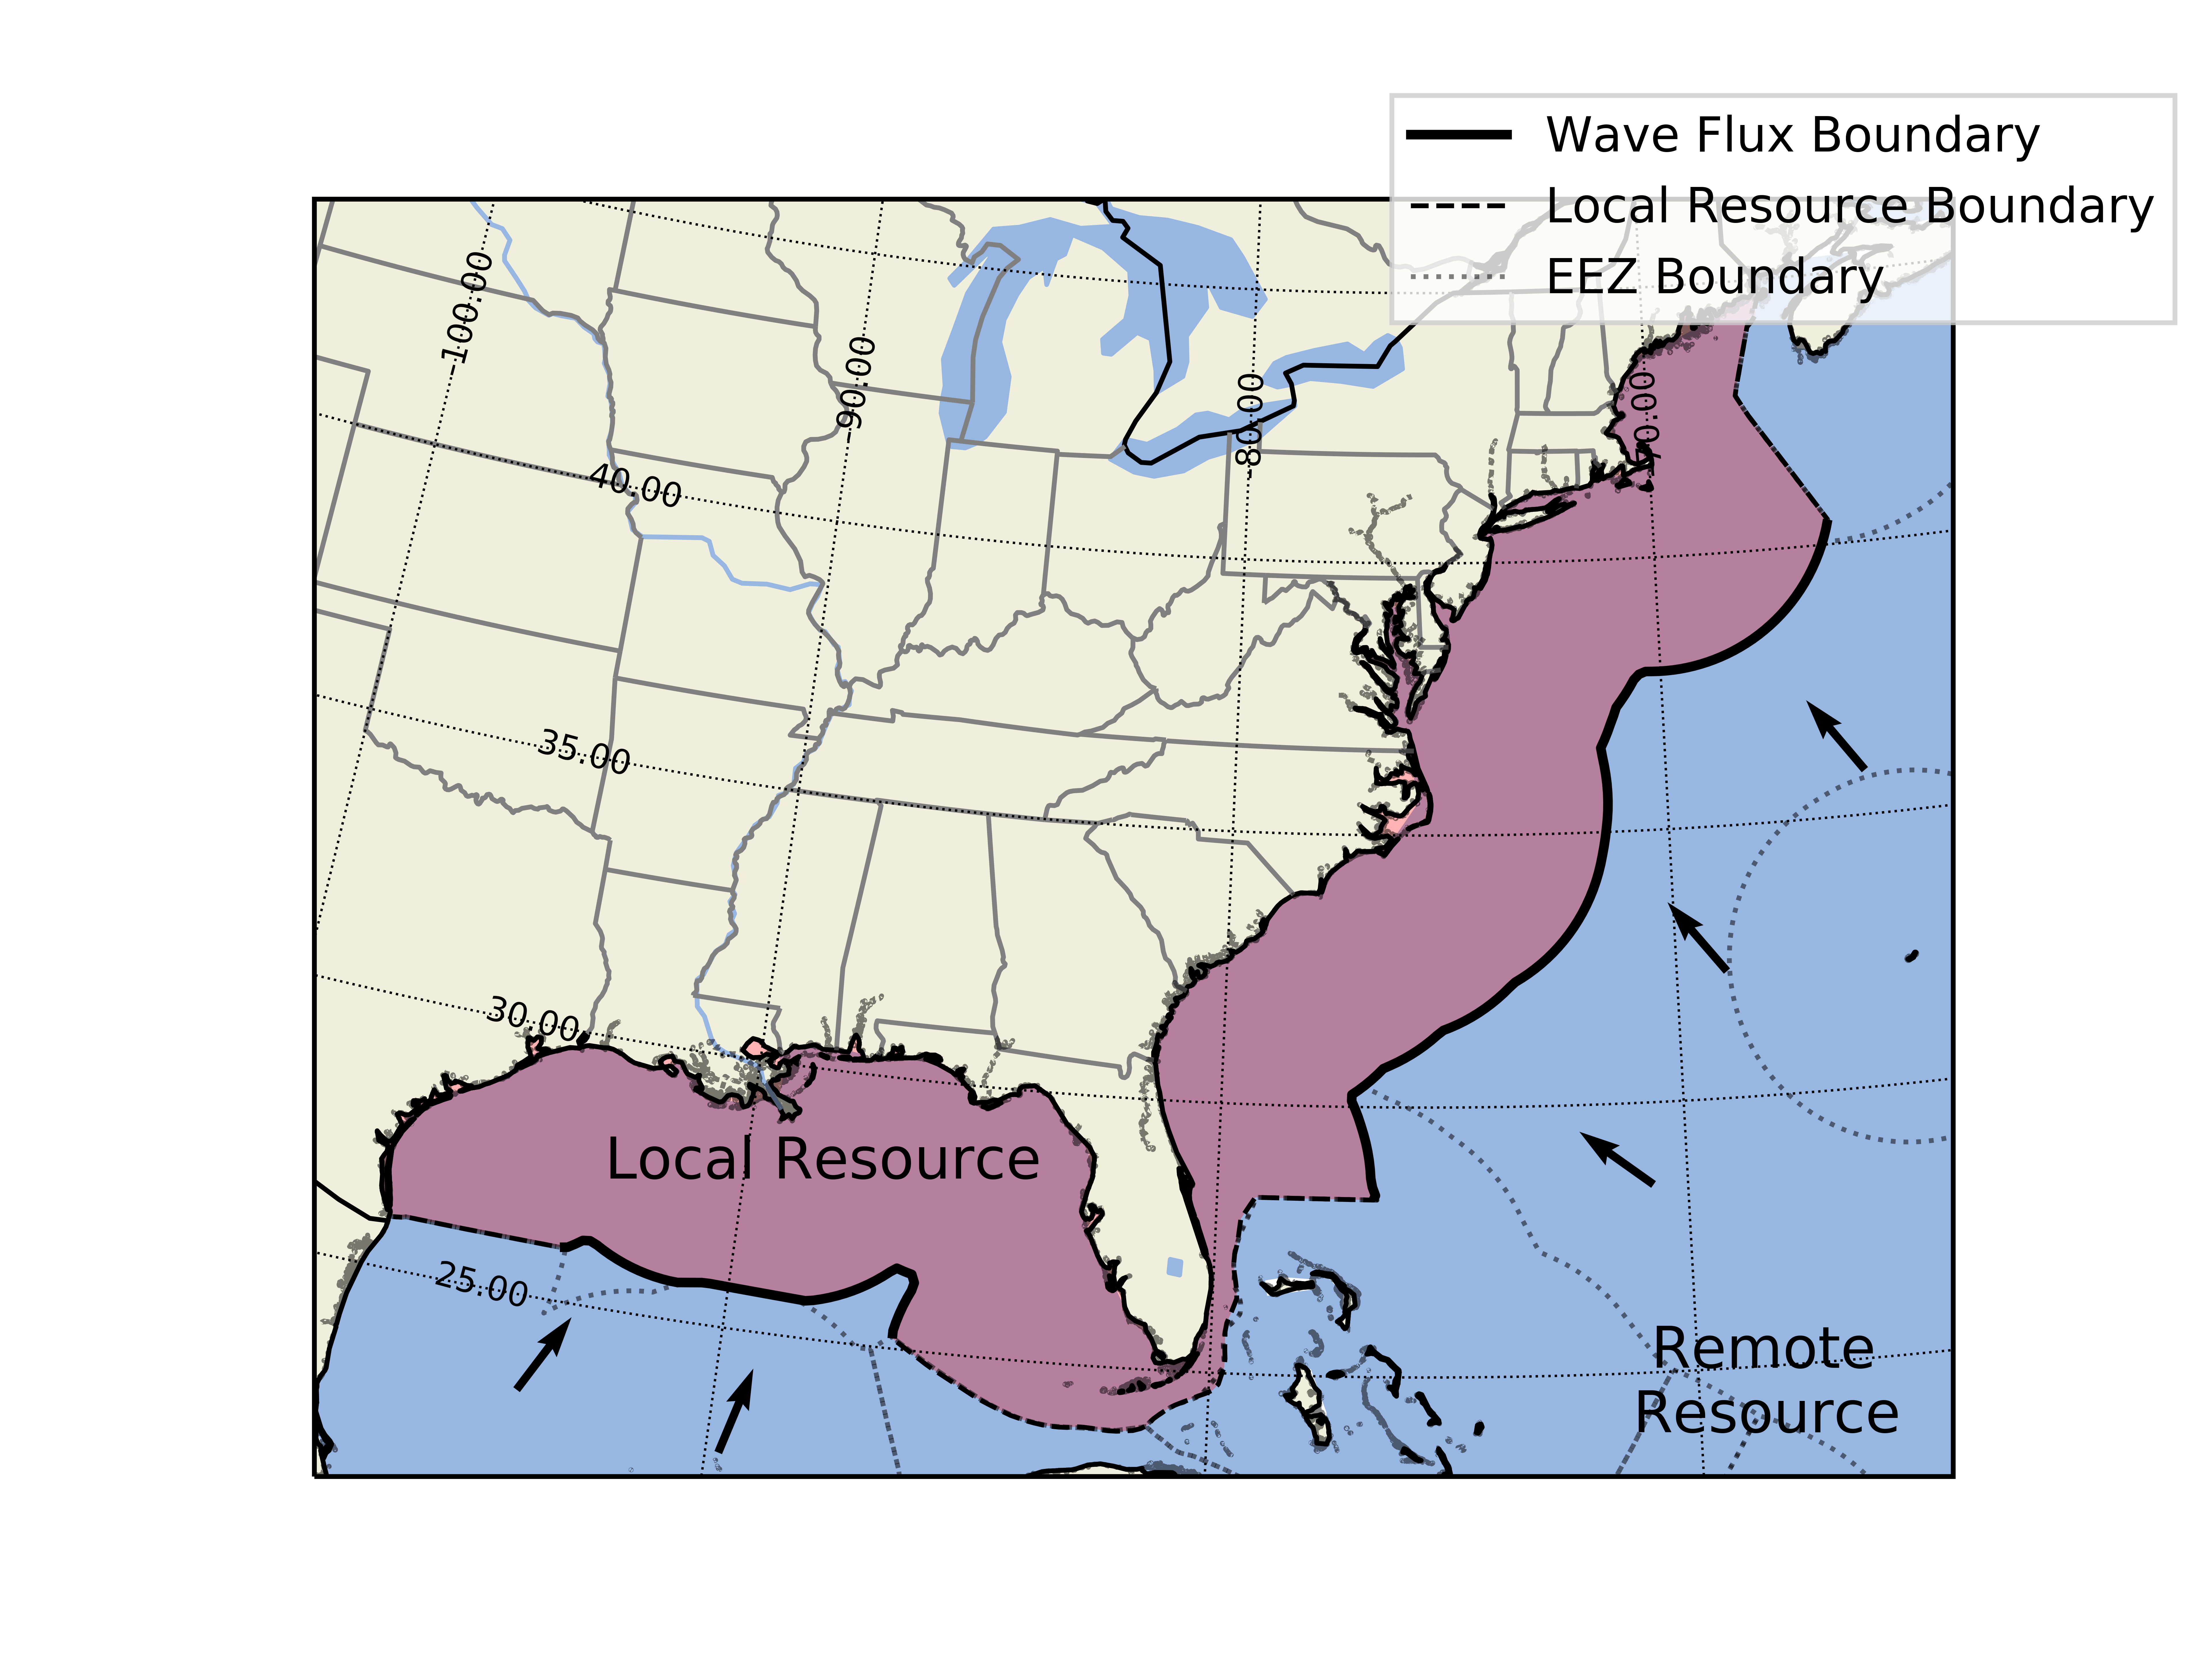
\includegraphics[width=0.7\textwidth]{../fig/at_EEZ_resourcePlot}
    \caption{The U.S. EEZ along the east and gulf coasts (burgandy). The thick solid line separates the EEZ from the open ocean (where $R_R$ is calculated), and dashed lines are borders with other nation's EEZs.}
    \label{fig:at-EEZ}
\end{figure}


%%% Local Variables:
%%% TeX-master: "wave_res"
%%% End:
